%%% LaTeX Template: Article/Thesis/etc. with colored headings and special fonts
%%%
%%% Source: http://www.howtotex.com/
%%% Feel free to distribute this template, but please keep to referal to http://www.howtotex.com/ here.
%%% February 2011
%%%
%%% Modified January 2016 by CDM

%%%  Preamble
\documentclass[11pt,letterpaper]{article}
\usepackage[margin=1.0in]{geometry}
\usepackage[T1]{fontenc}
\usepackage[bitstream-charter]{mathdesign}
\usepackage[latin1]{inputenc}					
\usepackage{amsmath}						
\usepackage{xcolor}
\usepackage{cite}
\usepackage{hyphenat}
\usepackage{graphicx}
\usepackage{float}
\usepackage{subfigure}
\usepackage{sectsty}
\usepackage[compact]{titlesec} 
\usepackage[tablegrid]{vhistory}
\usepackage{pbox}
\usepackage{url}
\allsectionsfont{\color{accentcolor}\scshape\selectfont}

%%% Definitions
%%%%%%%%%%%%%%%%%%%%%%%%%%%%%%%%%%%%%%%%%%%%%%%%%%
% Change me to fit your team/semester information
\definecolor{accentcolor}{rgb}{0.0,0.0,0.5} 
\newcommand{\teamname}{Team TLC}               %just to fill the line
\newcommand{\productname}{Roam\_Bot}
\newcommand{\coursename}{CSE 4317: Senior Design II}
\newcommand{\semester}{Spring 2025}
\newcommand{\docname}{Detailed Design Specification}
\newcommand{\department}{Department of Computer Science \& Engineering}
\newcommand{\university}{The University of Texas at Arlington}
\newcommand{\authors}{Abubakar Kassim \\ Andrew Howard \\ Christopher Davis \\ Madison Gage \\ Raya Sultan \\}

%%% Headers and footers
\usepackage{fancyhdr}
	\pagestyle{fancy}						% Enabling the custom headers/footers
\usepackage{lastpage}	
	% Header (empty)
	\lhead{}
	\chead{}
	\rhead{}
	% Footer
	\lfoot{\footnotesize \teamname \ - \semester}
	\cfoot{}
	\rfoot{\footnotesize page \thepage\ of \pageref{LastPage}}	% "Page 1 of 2"
	\renewcommand{\headrulewidth}{0.0pt}
	\renewcommand{\footrulewidth}{0.4pt}

%%% Change the abstract environment
\usepackage[runin]{abstract}			% runin option for a run-in title
%\setlength\absleftindent{30pt}			% left margin
%\setlength\absrightindent{30pt}		% right margin
\abslabeldelim{\quad}	
\setlength{\abstitleskip}{-10pt}
\renewcommand{\abstractname}{}
\renewcommand{\abstracttextfont}{\color{accentcolor} \small \slshape}	% slanted text

%%% Start of the document
\begin{document}

%%% Cover sheet
{\centering \huge \color{accentcolor} \sc \textbf{\department \\ \university} \par} % department/university info
\vspace{1 in}
{\centering \huge \color{accentcolor} \sc \textbf{\docname \\ \coursename \\ \semester} \par} % doc/semester info
\vspace{0.1 in} % spacing before cover sheet image
%%%%%%%%%%%%%%%%%%%%%%%%%%%%%%%%%%%%%%%%%%%%%%%%%%%%%%%%%%%%%%%%%%%%%%%%%%%%
%   Change the graphic here. Put your image in the 'images' folder
%   and update the name from 'images/test_image' to your image name
\begin{figure}[h!]
	\centering
   	
\includegraphics[width=0.60\textwidth]{images/logo.png}
\end{figure}
\vspace{0.1 in} % spacing after cover sheet image, before team/product info
{\centering \huge \color{accentcolor} \sc \textbf{\teamname \\ \productname} \par}
\vspace{0.1 in} % spacing before team members
{\centering \large \sc \textbf{\authors} \par}
\newpage


%\vspace{1 in}
%\centerline{January 13th, 2012}
%\newpage

%%% Revision History
\begin{versionhistory}
    \vhEntry{0.1}{2.4.2025}{CC}{Document Creation}
    \vhEntry{0.2}{2.25.2025}{AH}{Added Introduction Information}
    \vhEntry{0.3}{2.27.2025}{CD|RS|AK|AH}{Added Layer Information}
    % \vhEntry{0.3}{1.12.2016}{AT|GH}{release candidate 1}
    % \vhEntry{0.4}{1.20.2016}{AT|GH|CB}{official release}
    % \vhEntry{0.5}{1.31.2016}{AL}{added design review requests}
    \vhEntry{1.0}{2.28.2025}{CD|RS|MG|AK|AH}{Official Release}
    \vhEntry{1.1}{4.30.2025}{AK}{Updated Layer Information}
    \vhEntry{2.0}{4.30.2025}{CD|RS|MG|AK|AH}{Official Release}
\end{versionhistory}
\newpage

%%% Table of contents
\setcounter{tocdepth}{2}
\tableofcontents
\newpage

%%% List of figures and tables (optional)
\listoffigures
\newpage

%%% Document sections

\section{Introduction}
% Your introduction should provide a brief overview of the product concept and a reference to the requirement specification and architectural design documents in 1 or 2 paragraphs. The purpose is to provide the reader with the location of relevant background material that lead to the design details presented in this document.

The RoamBot should assist with learning to implement autonomous system software through real test simulations. This will be achieved using actual robotic systems. The overall design is controlled by a Raspberry Pi, which acts as the host connecting the different components of the rover. The first section describes the rover's motion and functionality. The second section entails the interface which allows users to upload their algorithm or manually control the rover. The third section is about the path-finding function, which dictates where the rover can move with the use of LIDAR and other sensors.

\newpage

\section{System Overview}
This section should reintroduce the full data flow diagram from the architectural specification, and discuss at a high level the purpose of each layer. You do not need to include a subsection for each layer, a 1 - 2 paragraph recap is sufficient.

\begin{figure}[h!]
	\centering
 	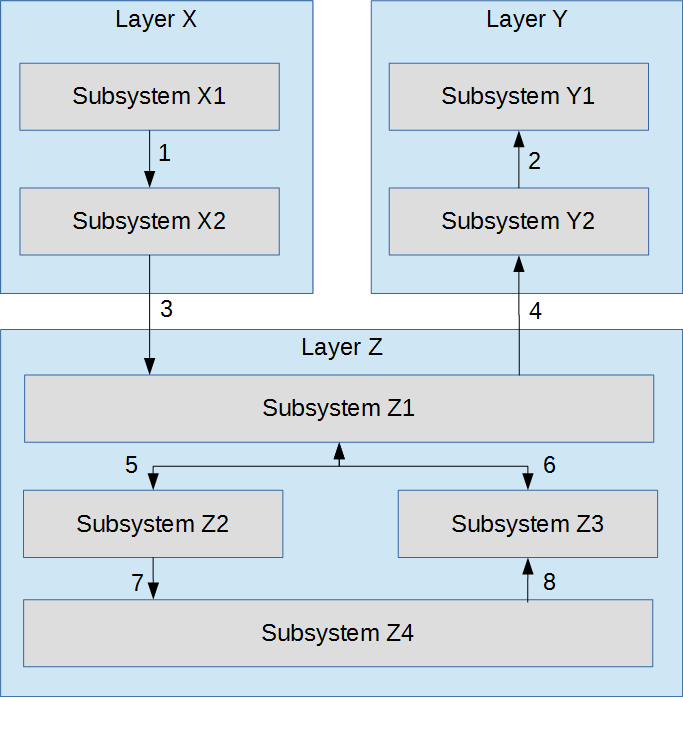
\includegraphics[width=0.90\textwidth]{images/data_flow}
 \caption{System architecture}
\end{figure}

\newpage
%\section{Subsystem Definitions \& Data Flow}
%% This section breaks down your layer abstraction to another level of detail. Here you grapically represent the logical subsytems that compose each layer and show the interactions/interfaces between those subsystems. A subsystem can be thought of as a programming unit that implements one of the major functions of the layer. It, therefore, has data elements that serve as source/sinks for other subsystems. The logical data elements that flow between subsystems need to be explicitly defined at this point, beginning with a data flow-like diagram based on the block diagram.

%%%%%%%%%%%%%%%%%%%%%%%%%%%%%%%%%%%%%%%%%%%%%%%%%%%%%%%%%%%%%%%%%%%%%%%%%%%%
%   Change the graphic here. Put your image in the 'images' folder
%   and update the name from 'images/test_image' to your image name
\begin{figure}[h!]
	\centering
 	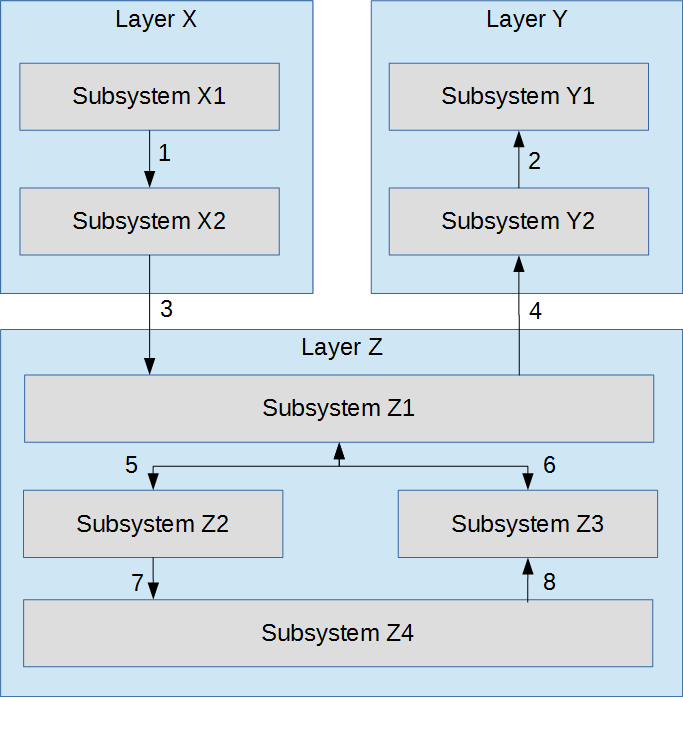
\includegraphics[width=\textwidth]{images/data_flow}
 \caption{A simple data flow diagram} % Be sure to change the caption!
\end{figure}

\newpage
\section{Movement Layer Subsystems}
%%%%%%%%%%%%%%%%%%%%%%%%%%%%%%%%%%%%%%%%%%%%%%%%%%
%% Layer Overview
%%%%%%%%%%%%%%%%%%%%%%%%%%%%%%%%%%%%%%%%%%%%%%%%%%
% In this section, the layer is described in terms of the hardware and software design. Specific implementation details, such as hardware components, programming languages, software dependencies, operating systems, etc. should be discussed. Any unnecessary items can be ommitted (for example, a pure software module without any specific hardware should not include a hardware subsection). The organization, titles, and content of the sections below can be modified as necessary for the project.
The Movement Subsystem controls the rover's motion by managing speed, direction, and collision avoidance. It receives navigation commands from the Raspberry Pi and sends signals for motor control, ensuring responsive navigation.

%%%%%%%%%%%%%%%%%%%%%%%%%%%%%%%%%%%%%%%%%%%%%%%%%%
%% Layer Description
%%%%%%%%%%%%%%%%%%%%%%%%%%%%%%%%%%%%%%%%%%%%%%%%%%

% \subsection{Layer Hardware}
% A description of any involved hardware components for the layer. For example, if each subsystem is a software process running on an embedded computer, discuss the specifics of that device here. Do not list a hardware component that only exists at the subsystem level (include it in the following sections).

% \subsection{Layer Operating System}
% A description of any operating systems required by the layer.

% \subsection{Layer Software Dependencies}
% A description of any software dependencies (libraries, frameworks, etc) required by the layer.

%%%%%%%%%%%%%%%%%%%%%%%%%%%%%%%%%%%%%%%%%%%%%%%%%%
%% Subsystem X - Template
%%%%%%%%%%%%%%%%%%%%%%%%%%%%%%%%%%%%%%%%%%%%%%%%%%

% \subsection{Subsystem X}
% Descibe at a high level the purpose and basic design of this subsystem. Is it a piece of hardware, a class, a web service, or something else? Note that each of the subsystem items below are meant to be specific to that subystem and not a repeat of anything discussed above for the overall layer.

% \begin{figure}[h!]
% 	\centering
%  	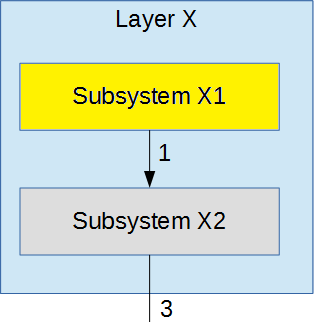
\includegraphics[width=0.60\textwidth]{images/subsystem}
%  \caption{Example subsystem description diagram}
% \end{figure}

% \subsubsection{Subsystem Hardware}
% A description of any involved hardware components for the subsystem.

% \subsubsection{Subsystem Operating System}
% A description of any operating systems required by the subsystem.

% \subsubsection{Subsystem Software Dependencies}
% A description of any software dependencies (libraries, frameworks, design software for mechanical parts or circuits, etc) required by the subsystem.

% \subsubsection{Subsystem Programming Languages}
% A description of any programming languages used by the subsystem.

% \subsubsection{Subsystem Data Structures}
% A description of any classes or other data structures that are worth discussing for the subsystem. For example, data being transmitted from a microcontroller to a PC via USB should be first be assembled into packets. What is the structure of the packets?

% \subsubsection{Subsystem Data Processing}
% A description of any algorithms or processing strategies that are worth discussing for the subsystem. If you are implementing a well-known algorithm, list it. If it is something unique to this project, discuss it in greater detail.



%%%%%%%%%%%%%%%%%%%%%%%%%%%%%%%%%%%%%%%%%%%%%%%%%%
%% Subsystem 1 - Microcontroller
%%%%%%%%%%%%%%%%%%%%%%%%%%%%%%%%%%%%%%%%%%%%%%%%%%

\subsection{Microcontroller}
The microcontroller \cite{TM4C} is a hardware component responsible for processing commands and controlling the rover's movement. It manages communication between the control systems and the motor drivers, sending directional and speed commands. Additionally, it handles sensor inputs for obstacle detection and emergency stops, ensuring safe and efficient operation.

\begin{figure}[h!]
	\centering
 	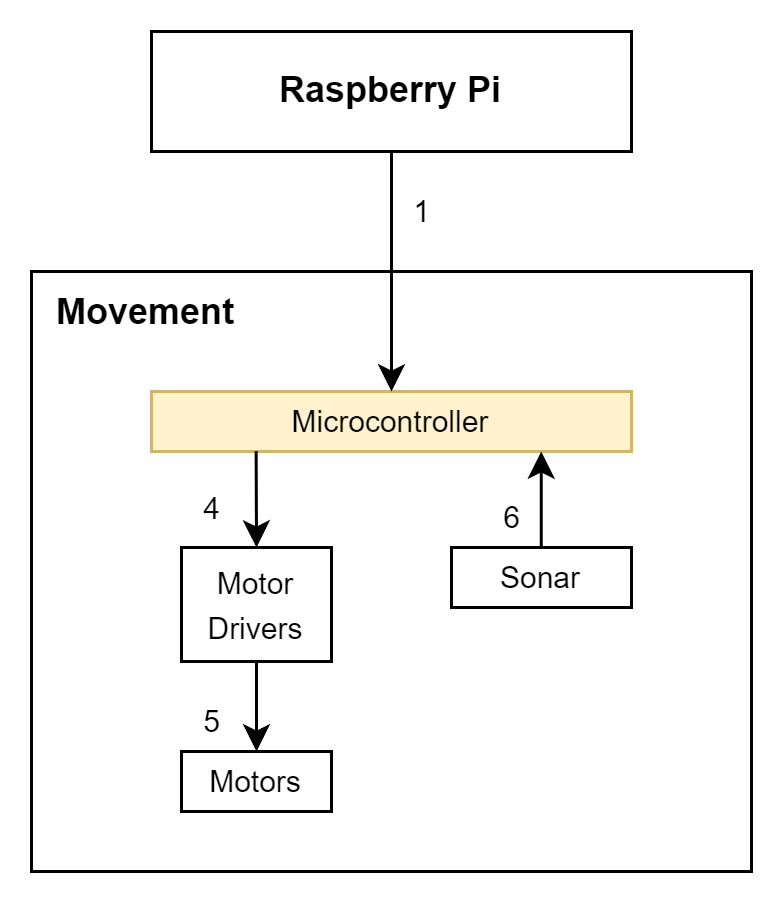
\includegraphics[width=0.60\textwidth]{images/movement/1_microcontroller.jpg}
 \caption{Movement Layer - Microcontroller Subsystem}
\end{figure}

\subsubsection{Subsystem Hardware}
\begin{itemize}
    \item TM4C RedBoard - A microcontroller with built-in UART and GPIO modules, responsible for processing motor control commands and handling sensor inputs (Figure \ref{fig:Movement Layer - Microcontroller Circuit}).
\end{itemize}

\subsubsection{Subsystem Software Dependencies}
TI Driver Library (Tivaware) - Provides low-level control over the TM4C RedBoard's peripherals, including UART and GPIO.

\subsubsection{Subsystem Programming Languages}
The TM4C RedBoard firmware uses C to implement the communication protocols and to control movement functions.

\subsubsection{Subsystem Data Structures}
\begin{itemize}
    \item (4x) 1-bit input GPIO control signals, one for each movement direction.
    \item 8-bit control packets are sent via UART to regulate each motor. Each packet consists of a single byte representing motor-specific commands such as speed and direction. Transmission occurs at 9600 baud with 5V, 8N1 settings, controlling one motor per packet.
\end{itemize}

\subsubsection{Subsystem Data Processing}
The microcontroller polls movement direction inputs every 100ms, capturing the required state and transmitting four motor control commands (one per motor).
\newpage



%%%%%%%%%%%%%%%%%%%%%%%%%%%%%%%%%%%%%%%%%%%%%%%%%%
%% Subsystem 2 - Motor Drivers
%%%%%%%%%%%%%%%%%%%%%%%%%%%%%%%%%%%%%%%%%%%%%%%%%%

\subsection{Motor Drivers}
The motor drivers \cite{Sabertooth} are hardware components that regulate power to the DC motors based on control packets received from the TM4C RedBoard. These are Sabertooth controllers that process incoming commands to adjust motor speed and direction. They ensure efficient and precise movement of the rover.

\begin{figure}[h!]
	\centering
 	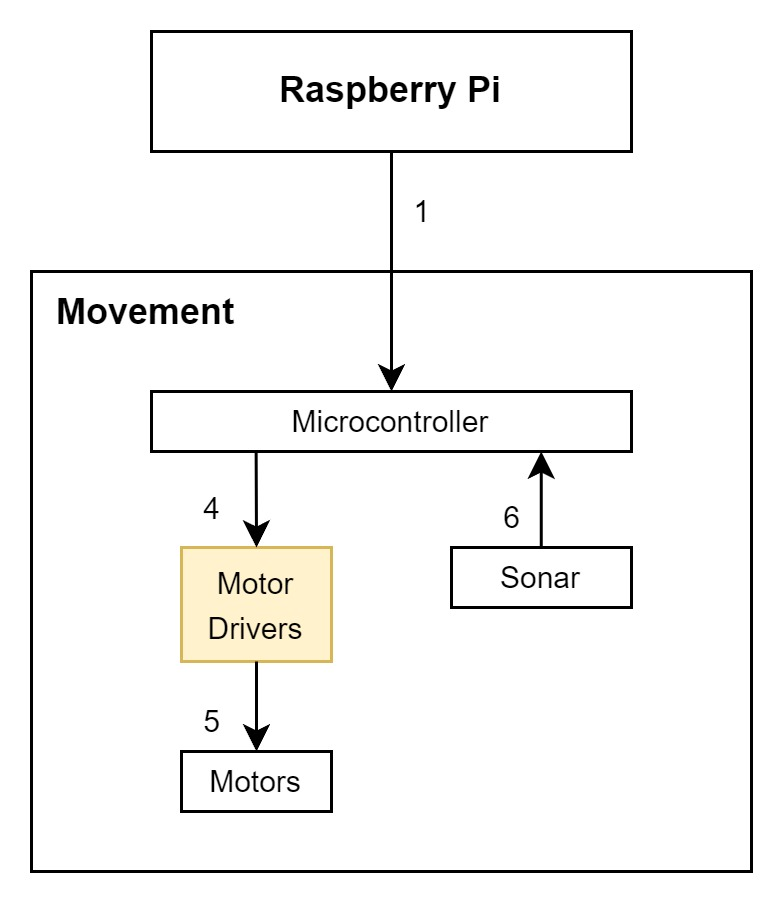
\includegraphics[width=0.60\textwidth]{images/movement/2_motordriver.jpg}
 \caption{Movement Layer - Motor Drivers Subsystem}
\end{figure}

\subsubsection{Subsystem Hardware}
\begin{itemize}
    \item Two Sabertooth 2x25 Motor Controllers - High-performance dual motor drivers that receive UART commands from the TM4C RedBoard. Each controller independently drives two motors, enabling precise movement control (Figure \ref{fig:Movement Layer - Motor Drivers Circuit}).
\end{itemize}

\subsubsection{Subsystem Data Structures}
\begin{itemize}
    \item 8-bit control packets regulate motor operations. Each packet consists of a single byte representing speed and direction commands. The packets are received over UART at 9600 baud with 3.3V, 8N1 (1 start bit, 8 data bits, 1 stop bit) settings, controlling one motor per packet.
\end{itemize}

\subsubsection{Subsystem Data Processing}
Each Sabertooth controller processes incoming UART packets every 100ms. Two packets (one per motor) are received per controller, spaced 50us apart to ensure proper sequencing and avoid command overlap.
\newpage



%%%%%%%%%%%%%%%%%%%%%%%%%%%%%%%%%%%%%%%%%%%%%%%%%%
%% Subsystem - Motors
%%%%%%%%%%%%%%%%%%%%%%%%%%%%%%%%%%%%%%%%%%%%%%%%%%

\subsection{Motors}
The motors are the primary actuators responsible for the physical movement of the rover. These are high-performance DC motors controlled by the motor drivers to achieve the desired speed and direction. The motors receive regulated power from the motor drivers, ensuring smooth movement.

\begin{figure}[h!]
\centering
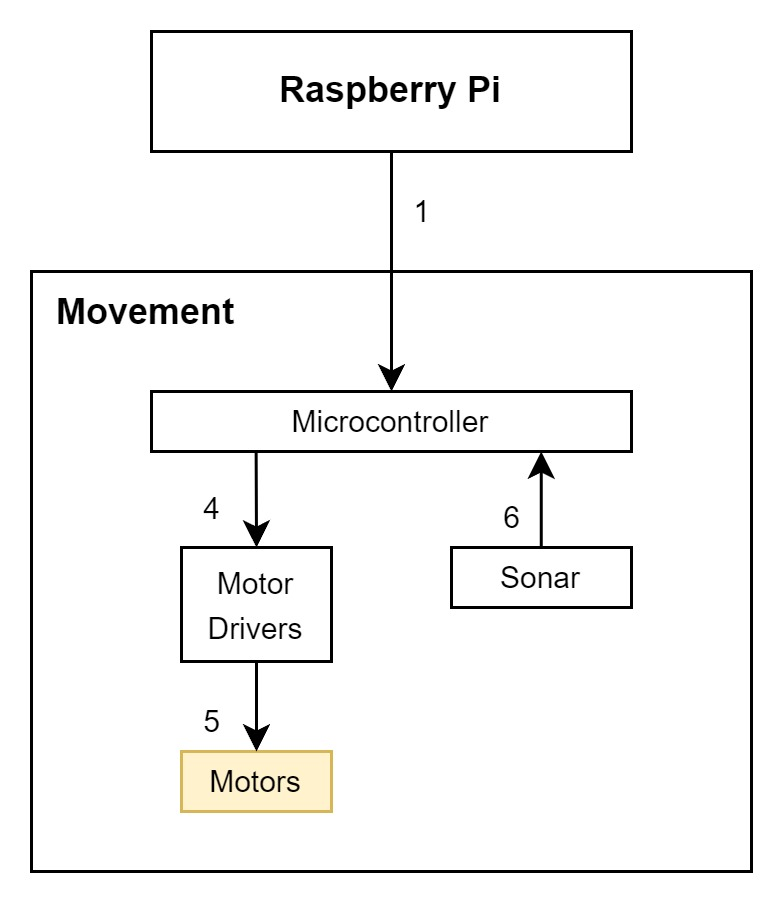
\includegraphics[width=0.60\textwidth]{images/movement/3_motors.jpg}
\caption{Movement Layer - Motors Subsystem}
\end{figure}

\subsubsection{Subsystem Hardware}
\begin{itemize}
\item Four DC Motors - Generate the mechanical power required for rover movement. The motors are grouped into front and rear pairs, each controlled independently by the motor drivers to regulate speed and direction.
\end{itemize}
\newpage



%%%%%%%%%%%%%%%%%%%%%%%%%%%%%%%%%%%%%%%%%%%%%%%%%%
%% Subsystem - Sonar (Last-Case Obstacle Detection)
%%%%%%%%%%%%%%%%%%%%%%%%%%%%%%%%%%%%%%%%%%%%%%%%%%\

\subsection{Sonar}
The Sonar subsystem utilizes ultrasonic sensors to detect obstacles in the rover's path. The system works by emitting sound waves and measuring the time it takes for the waves to bounce back after hitting an obstacle. The data is processed to determine the distance to the nearest object, enabling the rover to take last-minute actions to avoid collisions.

\begin{figure}[h!]
\centering
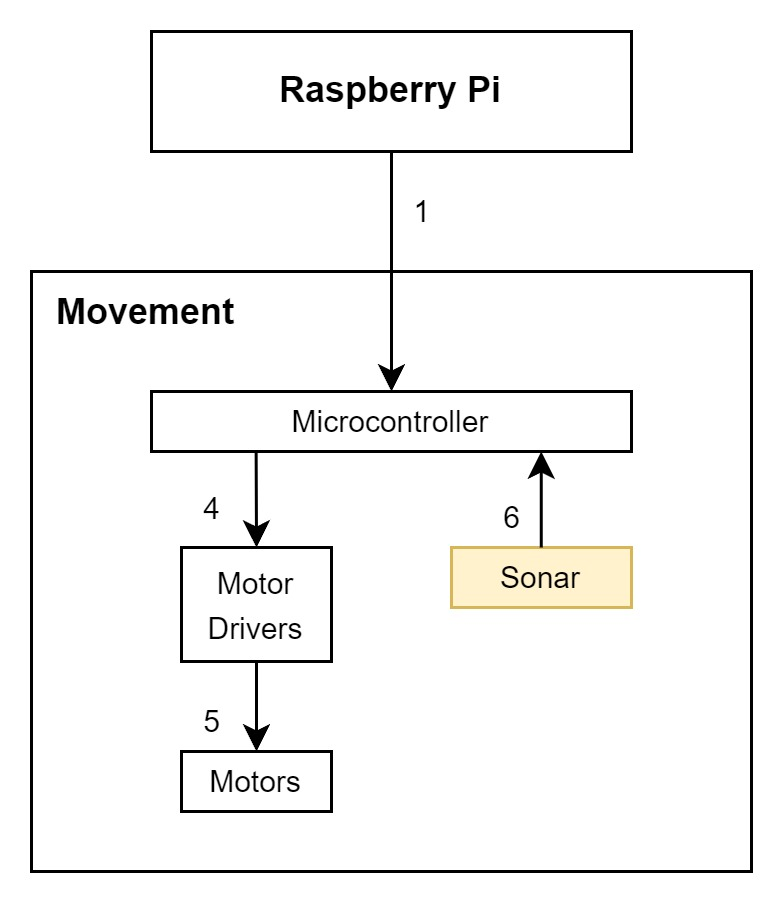
\includegraphics[width=0.60\textwidth]{images/movement/4_sonar.jpg}
\caption{Movement Layer - Sonar Subsystem}
\end{figure}

\subsubsection{Subsystem Hardware}
\begin{itemize}
    \item Ultrasonic Distance Sensor (HC-SR04) - Commonly used sensors that emit sound waves and listen for the echo, allowing for precise distance measurements to obstacles in the rover's path.
\end{itemize}

\subsubsection{Subsystem Data Structures}
\begin{itemize}
    \item 8-bit distance value (in centimeters) transmitted from the sensor to the microcontroller. This value represents the distance to the nearest obstacle detected by the sonar.
\end{itemize}

\subsubsection{Subsystem Data Processing}
The microcontroller sends a 10us pulse to the sensor's trigger pin, which causes the sensor to emit an ultrasonic wave. The time taken for the echo to return is measured to compute the distance. The system continuously polls the sensor at regular intervals (every 100ms) to update the obstacle detection distance. If an obstacle is detected within a defined threshold (50 cm), the rover will stop.

\newpage
\section{Pathfinding Layer Subsystems}
%%%%%%%%%%%%%%%%%%%%%%%%%%%%%%%%%%%%%%%%%%%%%%%%%%
%% Layer Overview
%%%%%%%%%%%%%%%%%%%%%%%%%%%%%%%%%%%%%%%%%%%%%%%%%%


%%%%%%%%%%%%%%%%%%%%%%%%%%%%%%%%%%%%%%%%%%%%%%%%%%
%% Subsystem X - Template
%%%%%%%%%%%%%%%%%%%%%%%%%%%%%%%%%%%%%%%%%%%%%%%%%%

% \subsection{Subsystem X}
% Descibe at a high level the purpose and basic design of this subsystem. Is it a piece of hardware, a class, a web service, or something else? Note that each of the subsystem items below are meant to be specific to that subystem and not a repeat of anything discussed above for the overall layer.

% \begin{figure}[h!]
% 	\centering
%  	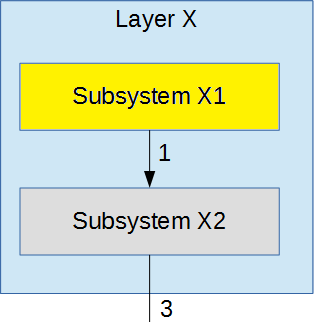
\includegraphics[width=0.60\textwidth]{images/subsystem}
%  \caption{Example subsystem description diagram}
% \end{figure}

% \subsubsection{Subsystem Hardware}
% A description of any involved hardware components for the subsystem.

% \subsubsection{Subsystem Operating System}
% A description of any operating systems required by the subsystem.

% \subsubsection{Subsystem Software Dependencies}
% A description of any software dependencies (libraries, frameworks, design software for mechanical parts or circuits, etc) required by the subsystem.

% \subsubsection{Subsystem Programming Languages}
% A description of any programming languages used by the subsystem.

% \subsubsection{Subsystem Data Structures}
% A description of any classes or other data structures that are worth discussing for the subsystem. For example, data being transmitted from a microcontroller to a PC via USB should be first be assembled into packets. What is the structure of the packets?

% \subsubsection{Subsystem Data Processing}
% A description of any algorithms or processing strategies that are worth discussing for the subsystem. If you are implementing a well-known algorithm, list it. If it is something unique to this project, discuss it in greater detail.



The Pathfinding Subsystem controls the rover's movement, by utilizing the rover's LIDAR to create a map of the terrain. The subsystem will than create a costmap grid, and than applying an A* pathfinding algorithm to find the most efficient and safest path.

\subsection{Navigation}
The Navigation system is a core component responsible for guiding the rover through its environment safely and efficiently. It combines sensor input, mapping, localization, and path planning to enable autonomous movement. Using real-time data from perception subsystems, the navigation system constructs a map of the surroundings, determines the rover's position within that map, and plans feasible routes to target destinations. It continuously updates the robot's trajectory to avoid obstacles and adapt to changes in the environment, ensuring smooth and collision-free traversal. This system is tightly integrated with motion control and localization components to maintain accurate positioning and responsive movement.

\begin{figure}[h!]
	\centering
 	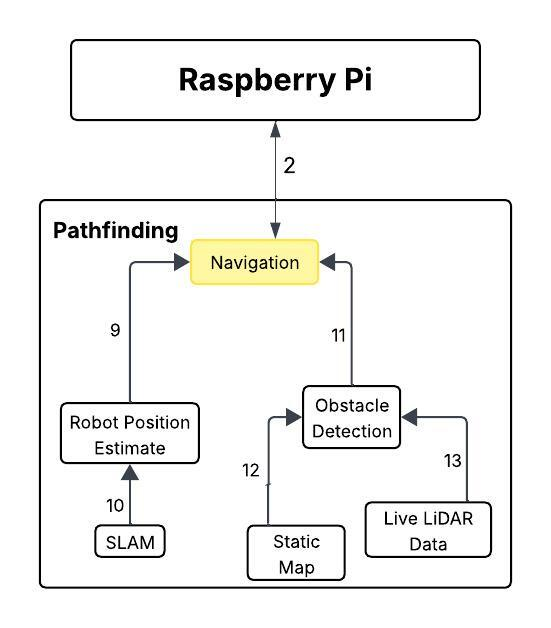
\includegraphics[width=0.60\textwidth]{images/pathfinding2nd/Data_Flow_Navigation.jpeg}
 \caption{Pathfinding Layer - LIDAR Subsystem}
\end{figure}


\subsubsection{Subsystem Hardware}
Slamtec RPLIDAR A1 - 360-degree laser range scanner. With a maximum range of 100 meters and a sampling frequency of a little over 2500 samples a second, measures distances and angles to create a 2D cloud point representation of the surroundings.

\subsubsection{Subsystem Operating System}
The navigation subsystem will be run on ROS2 Jazzy which requires Ubuntu 24.04 (Noble Numbat) or higher for compatibility. 

\subsubsection{Subsystem Dependencies}
The Navigation Subsystem uses Nav2 and ROS2 to develop the pathfinding algorithm and design the path for the rover to follow, and ROS2 to manage the robot's movements.

\subsubsection{Subsystem Programming Languages}
Nav2 is primarily implemented in C++ to ensure optimal compatibility with ROS2, which is also C++-
based. However, it also provides a Python API for additional flexibility.
\subsubsection{Subsystem Data Structures}
The pathfinding subsystem employs the A* algorithm due to its ability to determine the most optimal
path while maintaining lower computational overhead compared to alternative pathfinding methods.
\subsubsection{Subsystem Data Processing}
The pathfinding subsystem employs the A* algorithm due to its ability to determine the most optimal path while maintaining lower computational overhead compared to alternative pathfinding methods. (such as Djikstra, BFS)

\newpage

\subsection{Obstacle Detection}
The Obstacle Detection subsystem leverages the costmap generated by the Grid Management Subsystem to assess the robot's environment. It assigns a numerical value to each grid cell based on the proximity of surrounding objects, with higher values indicating closer objects and lower values representing areas free from obstacles.

\begin{figure}[h!]
	\centering
 	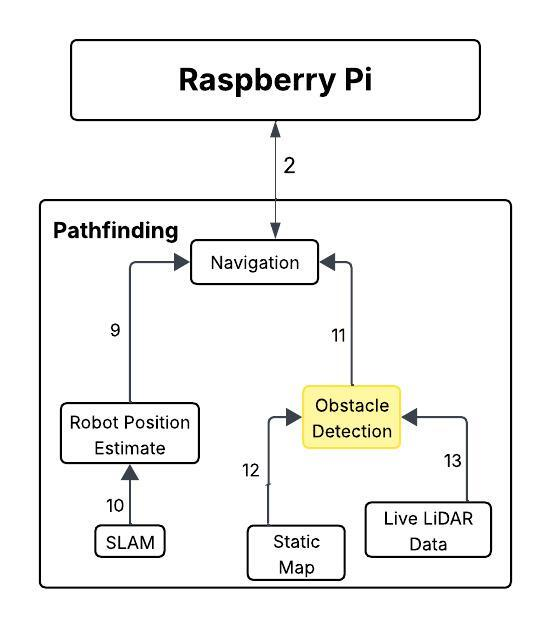
\includegraphics[width=0.60\textwidth]{images/pathfinding2nd/Data_Flow_ObstacleD.jpeg}
 \caption{Pathfinding Layer - Navigation Subsystem}
\end{figure}

%\subsubsection{Subsystem Hardware}
%The navigation software will be housed on the Raspberry Pi 5.
\subsubsection{Subsystem Operating System}
%A description of any operating systems required by the subsystem.
ROS2 Jazzy requires Ubuntu 24.04 (Noble Numbat) or higher for compatibility.
\subsubsection{Subsystem Software Dependencies}
%A description of any software dependencies (libraries, frameworks, design software for mechanical parts or circuits, etc) required by the subsystem.
The Obstacle Detection Subsystem uses Nav2 to develop the pathfinding algorithm and design the path for the rover to follow, and ROS2 to manage the robot's movements.

\subsubsection{Subsystem Programming Languages}
%A description of any programming languages used by %the subsystem.
Nav2 is primarily in C++, so it can better configure with ROS2 which is also in C++, but Nav2 does allow for a Python API.

\newpage

\subsection{Static Map}
The Static Map subsystem provides foundational spatial information for the rover's autonomous navigation. It consists of a pre-built occupancy grid defines known obstacles and traversable areas within a fixed environment, creating a costmap. In a ROS 2 and Nav2-based system, this map is loaded at runtime and used by the global planner to calculate optimal paths from the rover's current position to a designated goal. The static map enables efficient pathfinding by offering a reliable reference frame for localization and route generation.

\begin{figure}[h!]
	\centering
 	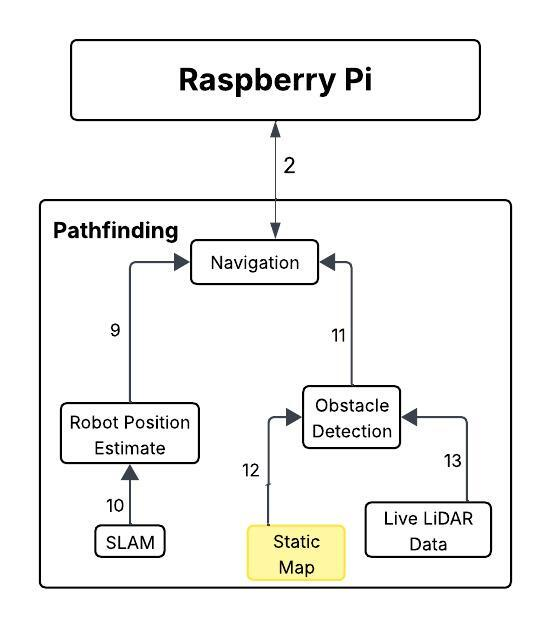
\includegraphics[width=0.60\textwidth]{images/pathfinding2nd/Data_Flow_StaticMap.jpeg}
 \caption{Pathfinding Layer - Static Map Subsystem}
\end{figure}


%\subsubsection{Subsystem Hardware}
%The Grid Management runs on Ros2 Jazzy which will be stored on the Raspberry Pi 5.
%\subsubsection{Subsystem Operating System}
%The Grid Management Subsystem will operate on ROS2 Jazzy, which requires Ubuntu 24.04 or later
\subsubsection{Subsystem Operating System}
Our Roam\_Bot utilizes a Slamtec RPLIDAR A1 - 360 Laser Range Scanner to create the static map
\subsubsection{Subsystem Software Dependencies}
The Static Map Subsystem uses Nav2 to to create the static map.
% \subsubsection{Subsystem Data Structures}

\newpage

\subsection{Live LiDAR Data}

The Live LiDAR Data subsystem provides real-time environmental awareness for the rover's navigation stack.  As the LIDAR sensor continuously scans the surroundings, it generates a dynamic stream of range measurements that are processed into a real-time occupancy grid.


\begin{figure}[h!]
	\centering
 	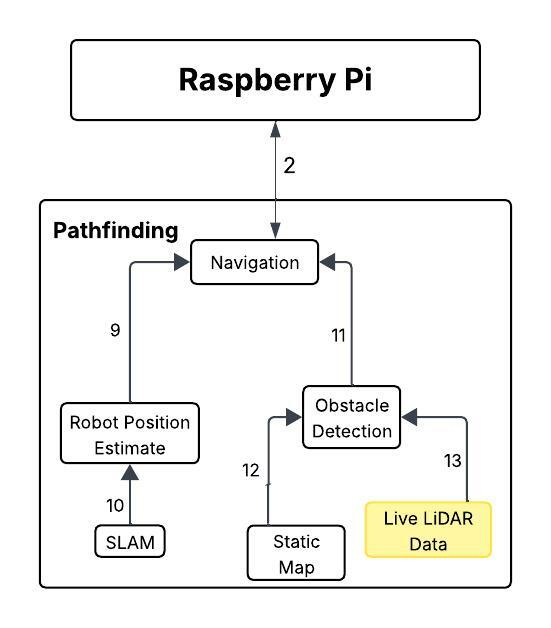
\includegraphics[width=0.60\textwidth]{images/pathfinding2nd/Data_Flow_LiveLiDAR.jpeg}
 \caption{Pathfinding Layer - Live LiDAR Data Subsystem}
\end{figure}

\subsubsection{Subsystem Hardware}
Our Roam\_Bot utilizes a Slamtec RPLIDAR A1 - 360 Laser Range Scanner. 


\subsubsection{Subsystem Operating System}
%A description of any operating systems required by the subsystem.
ROS2 Jazzy requires Ubuntu 24.04 (Noble Numbat) or higher for compatibility.

\newpage
\subsection{Robot Position Estimate}
% Descibe at a high level the purpose and basic design of this subsystem. Is it a piece of hardware, a class, a web service, or something else? Note that each of the subsystem items below are meant to be specific to that subystem and not a repeat of anything discussed above for the overall layer.
The robot position estimate subsystem is a software component responsible for determining the rover's location and orientation within its environment. It operates as part of the localization layer and integrates data from odometry, and LIDAR. The subsystem continuously fuses sensor inputs using probabilistic filtering techniques to maintain a stable and consistent position estimate, which is critical for navigation, path planning, and obstacle avoidance.

\begin{figure}[h!]
 	\centering
  	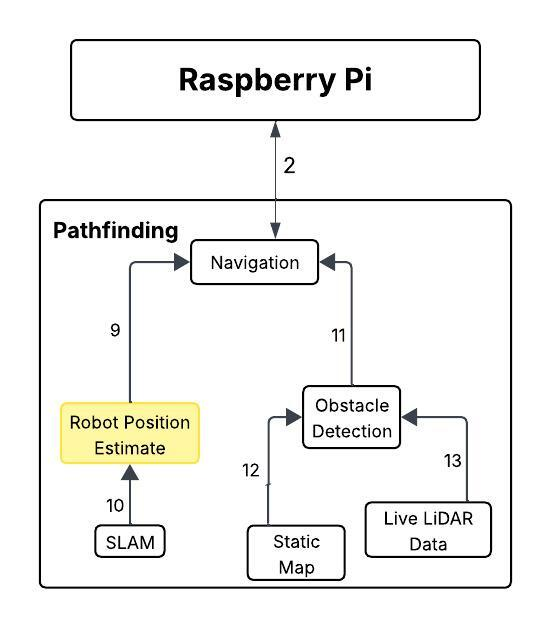
\includegraphics[width=0.60\textwidth]{images/pathfinding2nd/Data_Flow_RobotPosition.jpeg}
  \caption{Robot Position Estimate diagram}
 \end{figure}

 \subsubsection{Subsystem Hardware}
To create a position estimate for our Roam\_Bot we utilize our Slamtec RPLIDAR A1. 

\subsubsection{Subsystem Operating System}
ROS2 Jazzy requires Ubuntu 24.04 (Noble Numbat) or higher for compatibility.

\subsubsection{Subsystem Software Dependencies}
The Robot Position Estimate is calculated using ROS2 Jazzy and Nav2

\subsubsection{Subsystem Programming Languages}
the Robot Position Estimate is programmed in C++.

\newpage
\subsection{SLAM}
% Descibe at a high level the purpose and basic design of this subsystem. Is it a piece of hardware, a class, a web service, or something else? Note that each of the subsystem items below are meant to be specific to that subystem and not a repeat of anything discussed above for the overall layer.
The SLAM (Simultaneous Localization and Mapping) subsystem is a software module that enables the rover to navigate unknown environments by building a map while simultaneously estimating its position within it. As the robot moves, SLAM compares incoming sensor data to previous scans to update both its map and its own position. 

\begin{figure}[h!]
	\centering
 	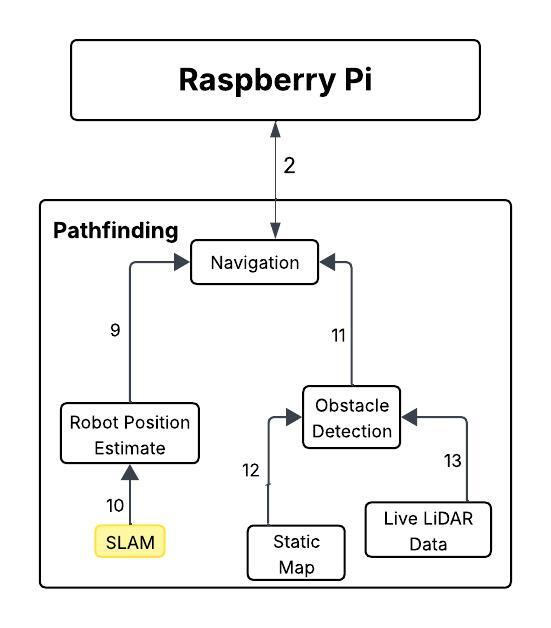
\includegraphics[width=0.60\textwidth]{images/pathfinding2nd/Data_Flow_SLAM.jpeg}
 \caption{SLAM diagram}
\end{figure}

\subsubsection{Subsystem Hardware}
SLAM relies on the SlamTec Lidar to derive the robot position estimate and map the floor,

\subsubsection{Subsystem Operating System}
% A description of any operating systems required by the subsystem.
ROS2 Jazzy requires Ubuntu 24.04 (Noble Numbat) or higher for compatibility.

\subsubsection{Subsystem Software Dependencies}
SLAM is calculated using ROS2 Jazzy and Nav2

\subsubsection{Subsystem Programming Languages}
% A description of any programming languages used by the subsystem.
Nav2 is primarily in C++, so it can better configure with ROS2 which is also in C++, but Nav2 does allow for a Python API.
\newpage
\section{Interface Layer Subsystems}
The interface subsystems of the RoamBot are responsible for processing user input and translating it into commands for the rover. These subsystems are implemented using C, C++, and Python and operate on the Raspberry Pi 5.

%In this section, the layer is described in terms of the hardware and software design. Specific implementation details, such as hardware components, programming languages, software dependencies, operating systems, etc. should be discussed. Any unnecessary items can be ommitted (for example, a pure software module without any specific hardware should not include a hardware subsection). The organization, titles, and content of the sections below can be modified as necessary for the project.

\subsection{Layer Hardware}
The Raspberry Pi 5 serves as the core interface hardware for the RoamBot, providing robust computational power with its quad-core ARM Cortex-A76 processor and 16GB of LPDDR4x RAM. It efficiently handles real-time pathfinding and decision-making processes. Additionally, its USB 3.0 ports and GPIO pins allow for direct connection to sensors and motor controllers.
%%%%%%%%%%%%%%% DEFINE MORE HARDWARE

\subsection{Layer Operating System}
The operating system used for the interface layer is Ubuntu 24.04, providing a stable environment for development and execution.

\subsection{Layer Software Dependencies}
The interface subsystems rely on the ROS2 framework for robotic control. These libraries are utilized for implementing communication protocols, control algorithms, and user input processing.

\subsubsection{Layer Programming Languages}
This layer is implemented using C, C++, and Python to efficiently process user commands and algorithm decisions and communicate with the motor control system.

\newpage

\subsection{UI Control}
The UI control subsystem serves as the top-level software interface for managing user interactions. It enables switching between direct user control and automated algorithmic control.

\begin{figure}[h!]
	\centering
 	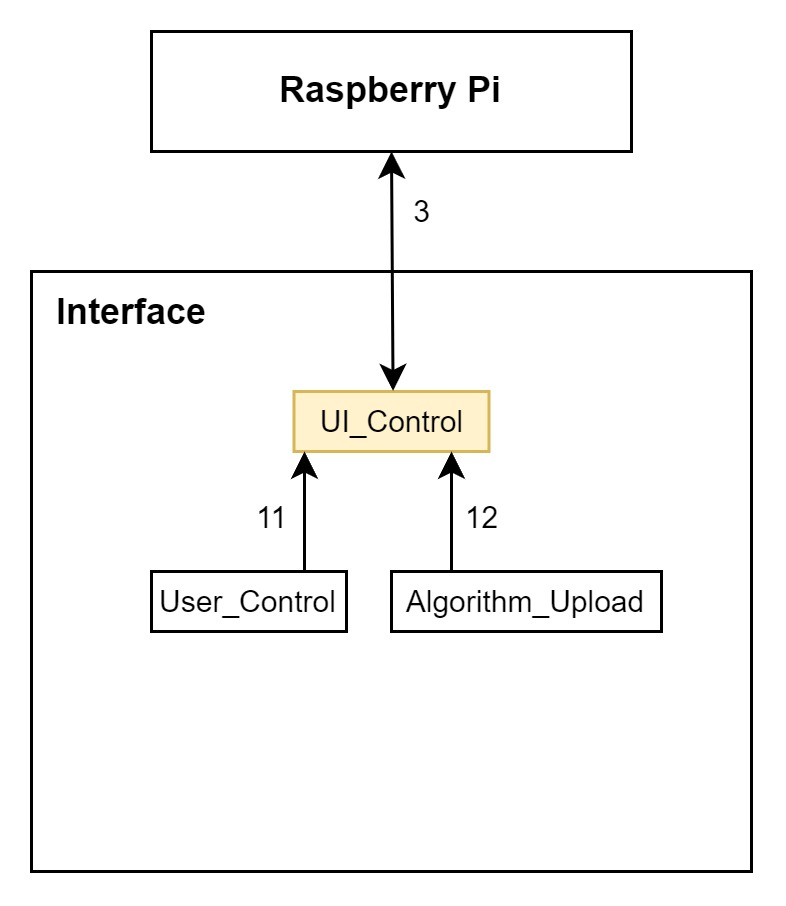
\includegraphics[width=0.60\textwidth]{images/interface/1_ui.jpg}
 \caption{Interface Layer - UI Control Subsystem}
\end{figure}

\subsubsection{Subsystem Data Structures}
The subsystem uses flag-based data structures to manage control mode status, with flags indicating whether the rover is in manual or autonomous mode. These flags are checked in real-time to determine which set of functions or commands should be executed.

\subsubsection{Subsystem Data Processing}
The UI control subsystem processes incoming user commands to switch between manual and automated modes by interpreting the mode. When a switch occurs, the system either routes input to the manual control system, allowing the user to directly guide the rover, or to the autonomous system, where the rover executes pre-programmed algorithms.

\newpage

\subsection{User Control}
The User Control subsystem allows direct manipulation of the RoamBot's movement in real-time. It processes immediate user inputs, and translates the input into motion instructions. This subsystem ensures that users have precise control over speed and direction, allowing manual operation when needed.

\begin{figure}[h!]
	\centering
 	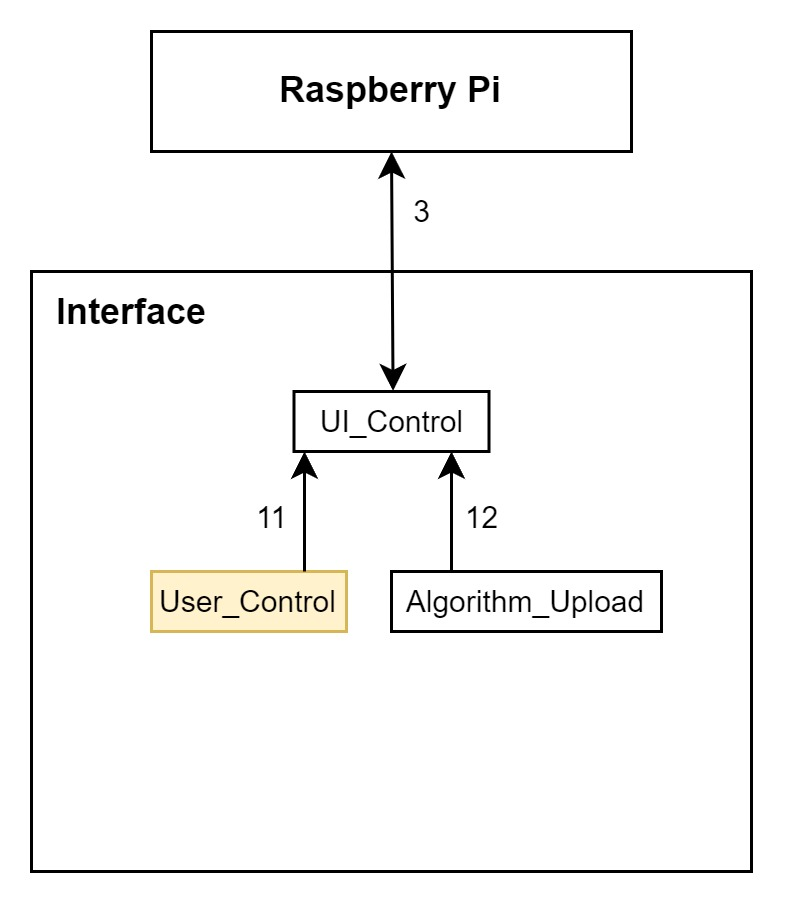
\includegraphics[width=0.60\textwidth]{images/interface/2_user.jpg}
 \caption{Interface Layer - User Control Subsystem}
\end{figure}

\subsubsection{Subsystem Programming Languages}
This subsystem is implemented using C, C++, and Python to efficiently process user commands and communicate with the motor control system.

\subsubsection{Subsystem Data Processing}
User inputs are converted into structured motion commands that control the rover's speed and direction. These commands are processed in real time to ensure responsiveness.

\newpage

\subsection{Algorithm Upload}
The Algorithm Upload subsystem allows users to upload pre-programmed pathfinding algorithms to enable autonomous navigation. It processes these algorithms and integrates them into the rover's control system, ensuring that the RoamBot can follow predefined paths without manual intervention.

\begin{figure}[h!]
	\centering
 	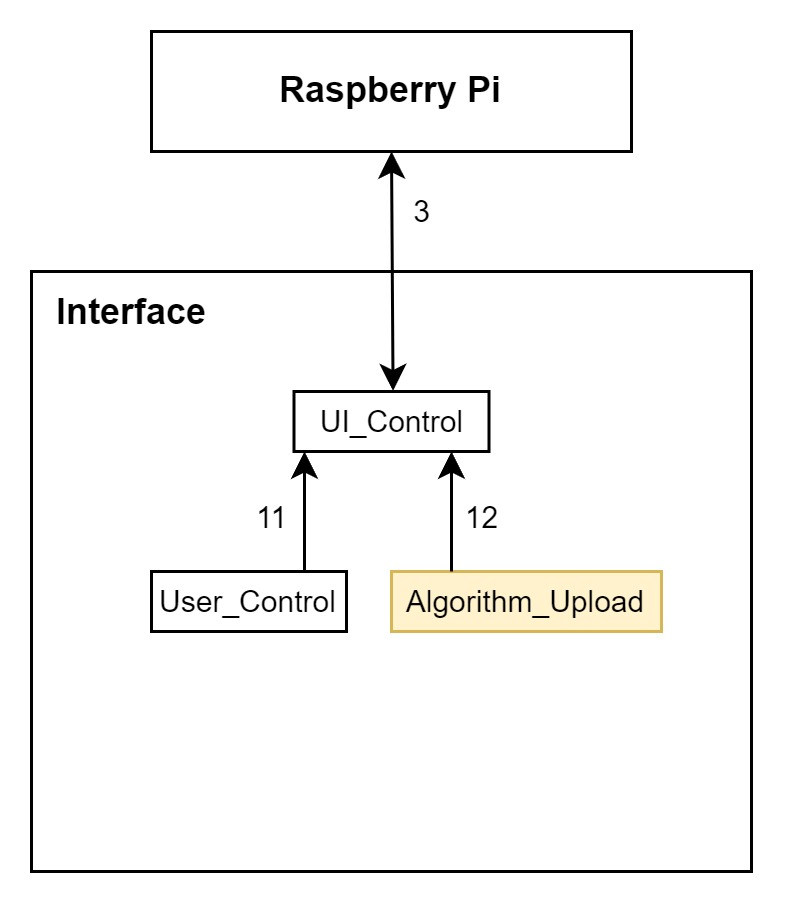
\includegraphics[width=0.60\textwidth]{images/interface/3_algorithm.jpg}
 \caption{Interface Layer - Algorithm Upload Subsystem}
\end{figure}

\subsubsection{Subsystem Data Structures}
The Algorithm Upload subsystem uses data structures like pathfinding grids or graphs to represent the environment, with nodes storing position and cost values values. The resulting path is stored as a sequence of waypoints.

\subsubsection{Subsystem Data Processing}
Data processing involves parsing the algorithm, running pathfinding algorithms like A* to generate a path, and converting it into motion commands. These commands are then sent as ROS2 messages to the motor control system for autonomous navigation.

\clearpage
\section{Appendix}
% Include any additional documents (CAD design, circuit schematics, etc) as an appendix as necessary.

\begin{figure}[h!]
	\centering
 	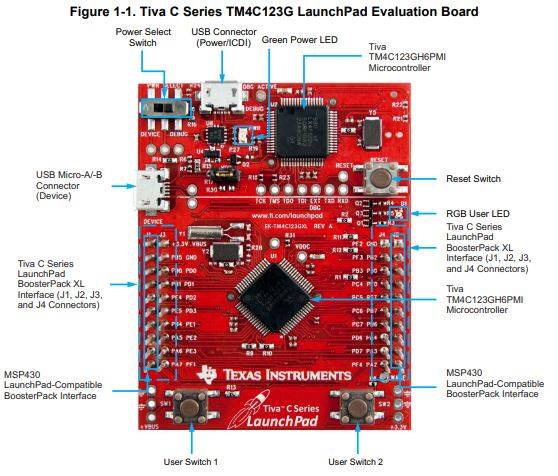
\includegraphics[width=1.00\textwidth]{images/circuits/1_redboard.jpg}
 \caption{Microcontroller Circuit}
 \label{fig:Microcontroller Circuit}
\end{figure}

\begin{figure}[h!]
	\centering
 	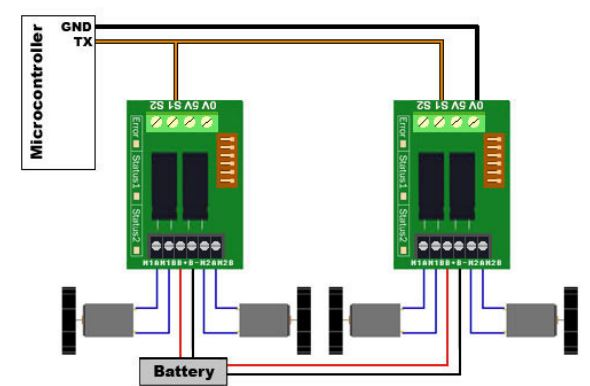
\includegraphics[width=1.00\textwidth]{images/circuits/2_sabertooth.JPG}
 \caption{Motor Drivers Circuit}
 \label{fig:Motor Drivers Circuit}
\end{figure}

\begin{figure}[h!]
	\centering
 	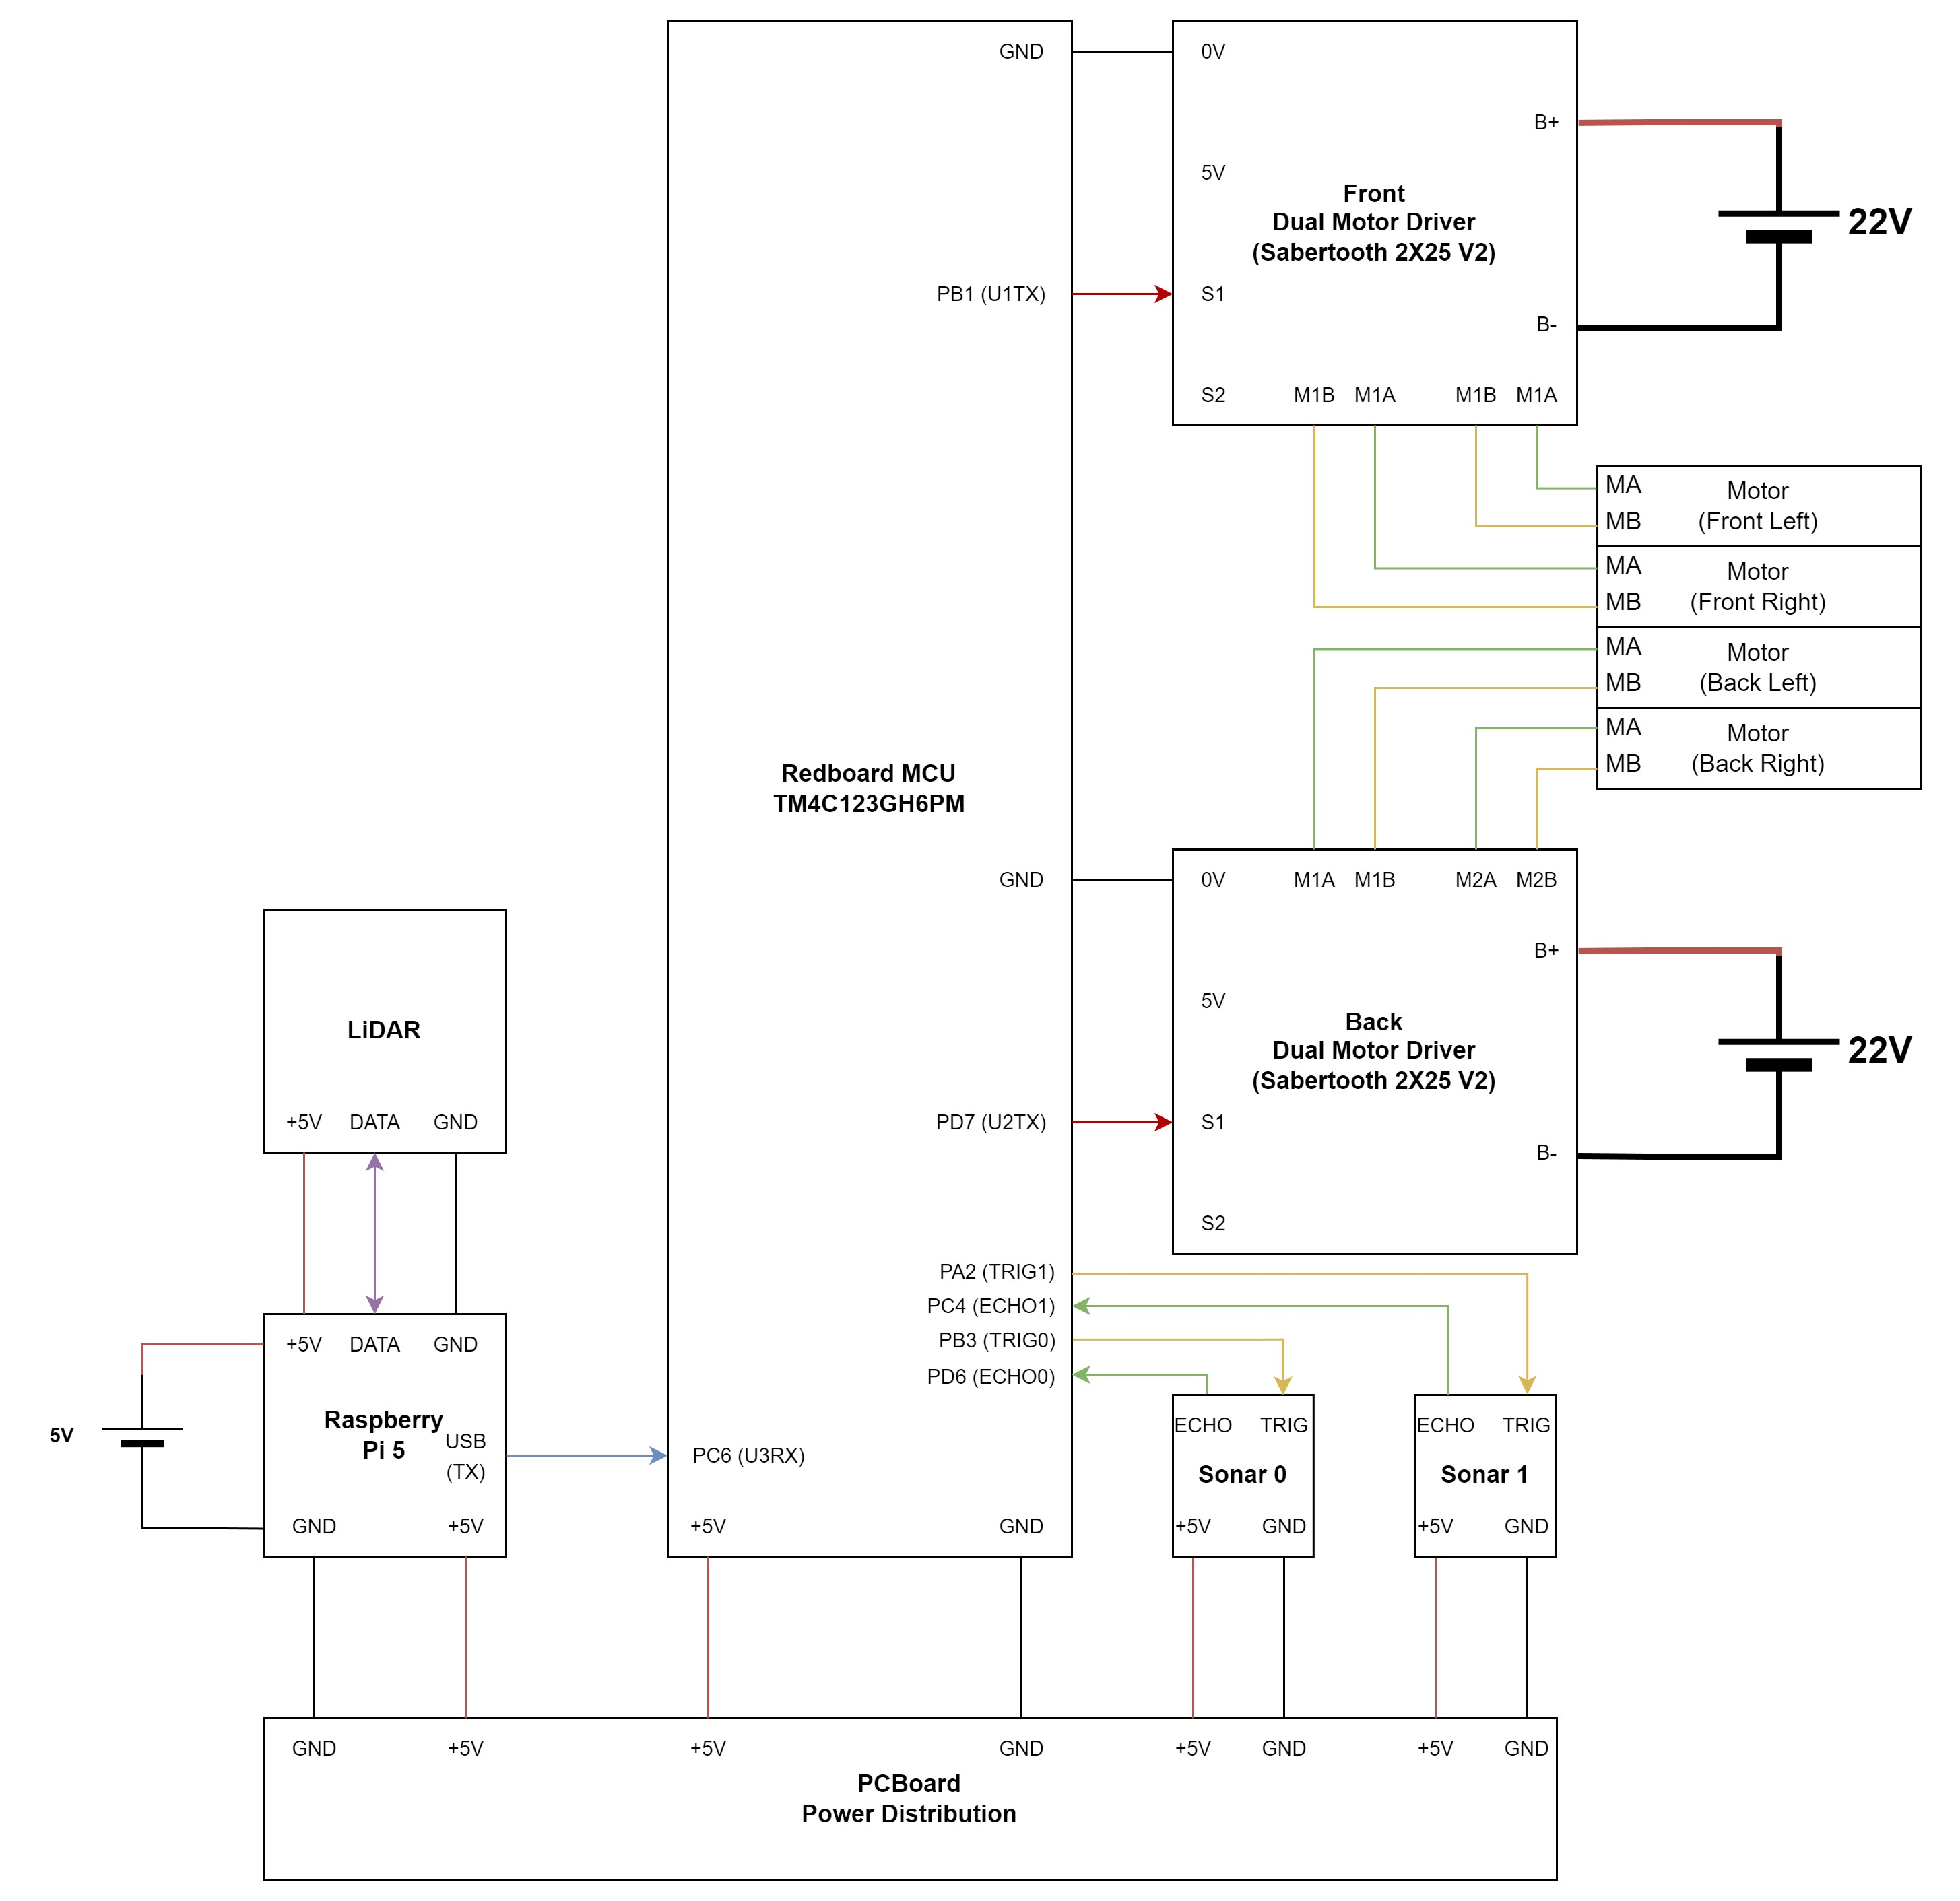
\includegraphics[width=1.00\textwidth]{images/circuits/3_pin_connections.jpg}
 \caption{Pin Connections}
 \label{fig:Pin Connections}
\end{figure}

\begin{figure}[h!]
	\centering
 	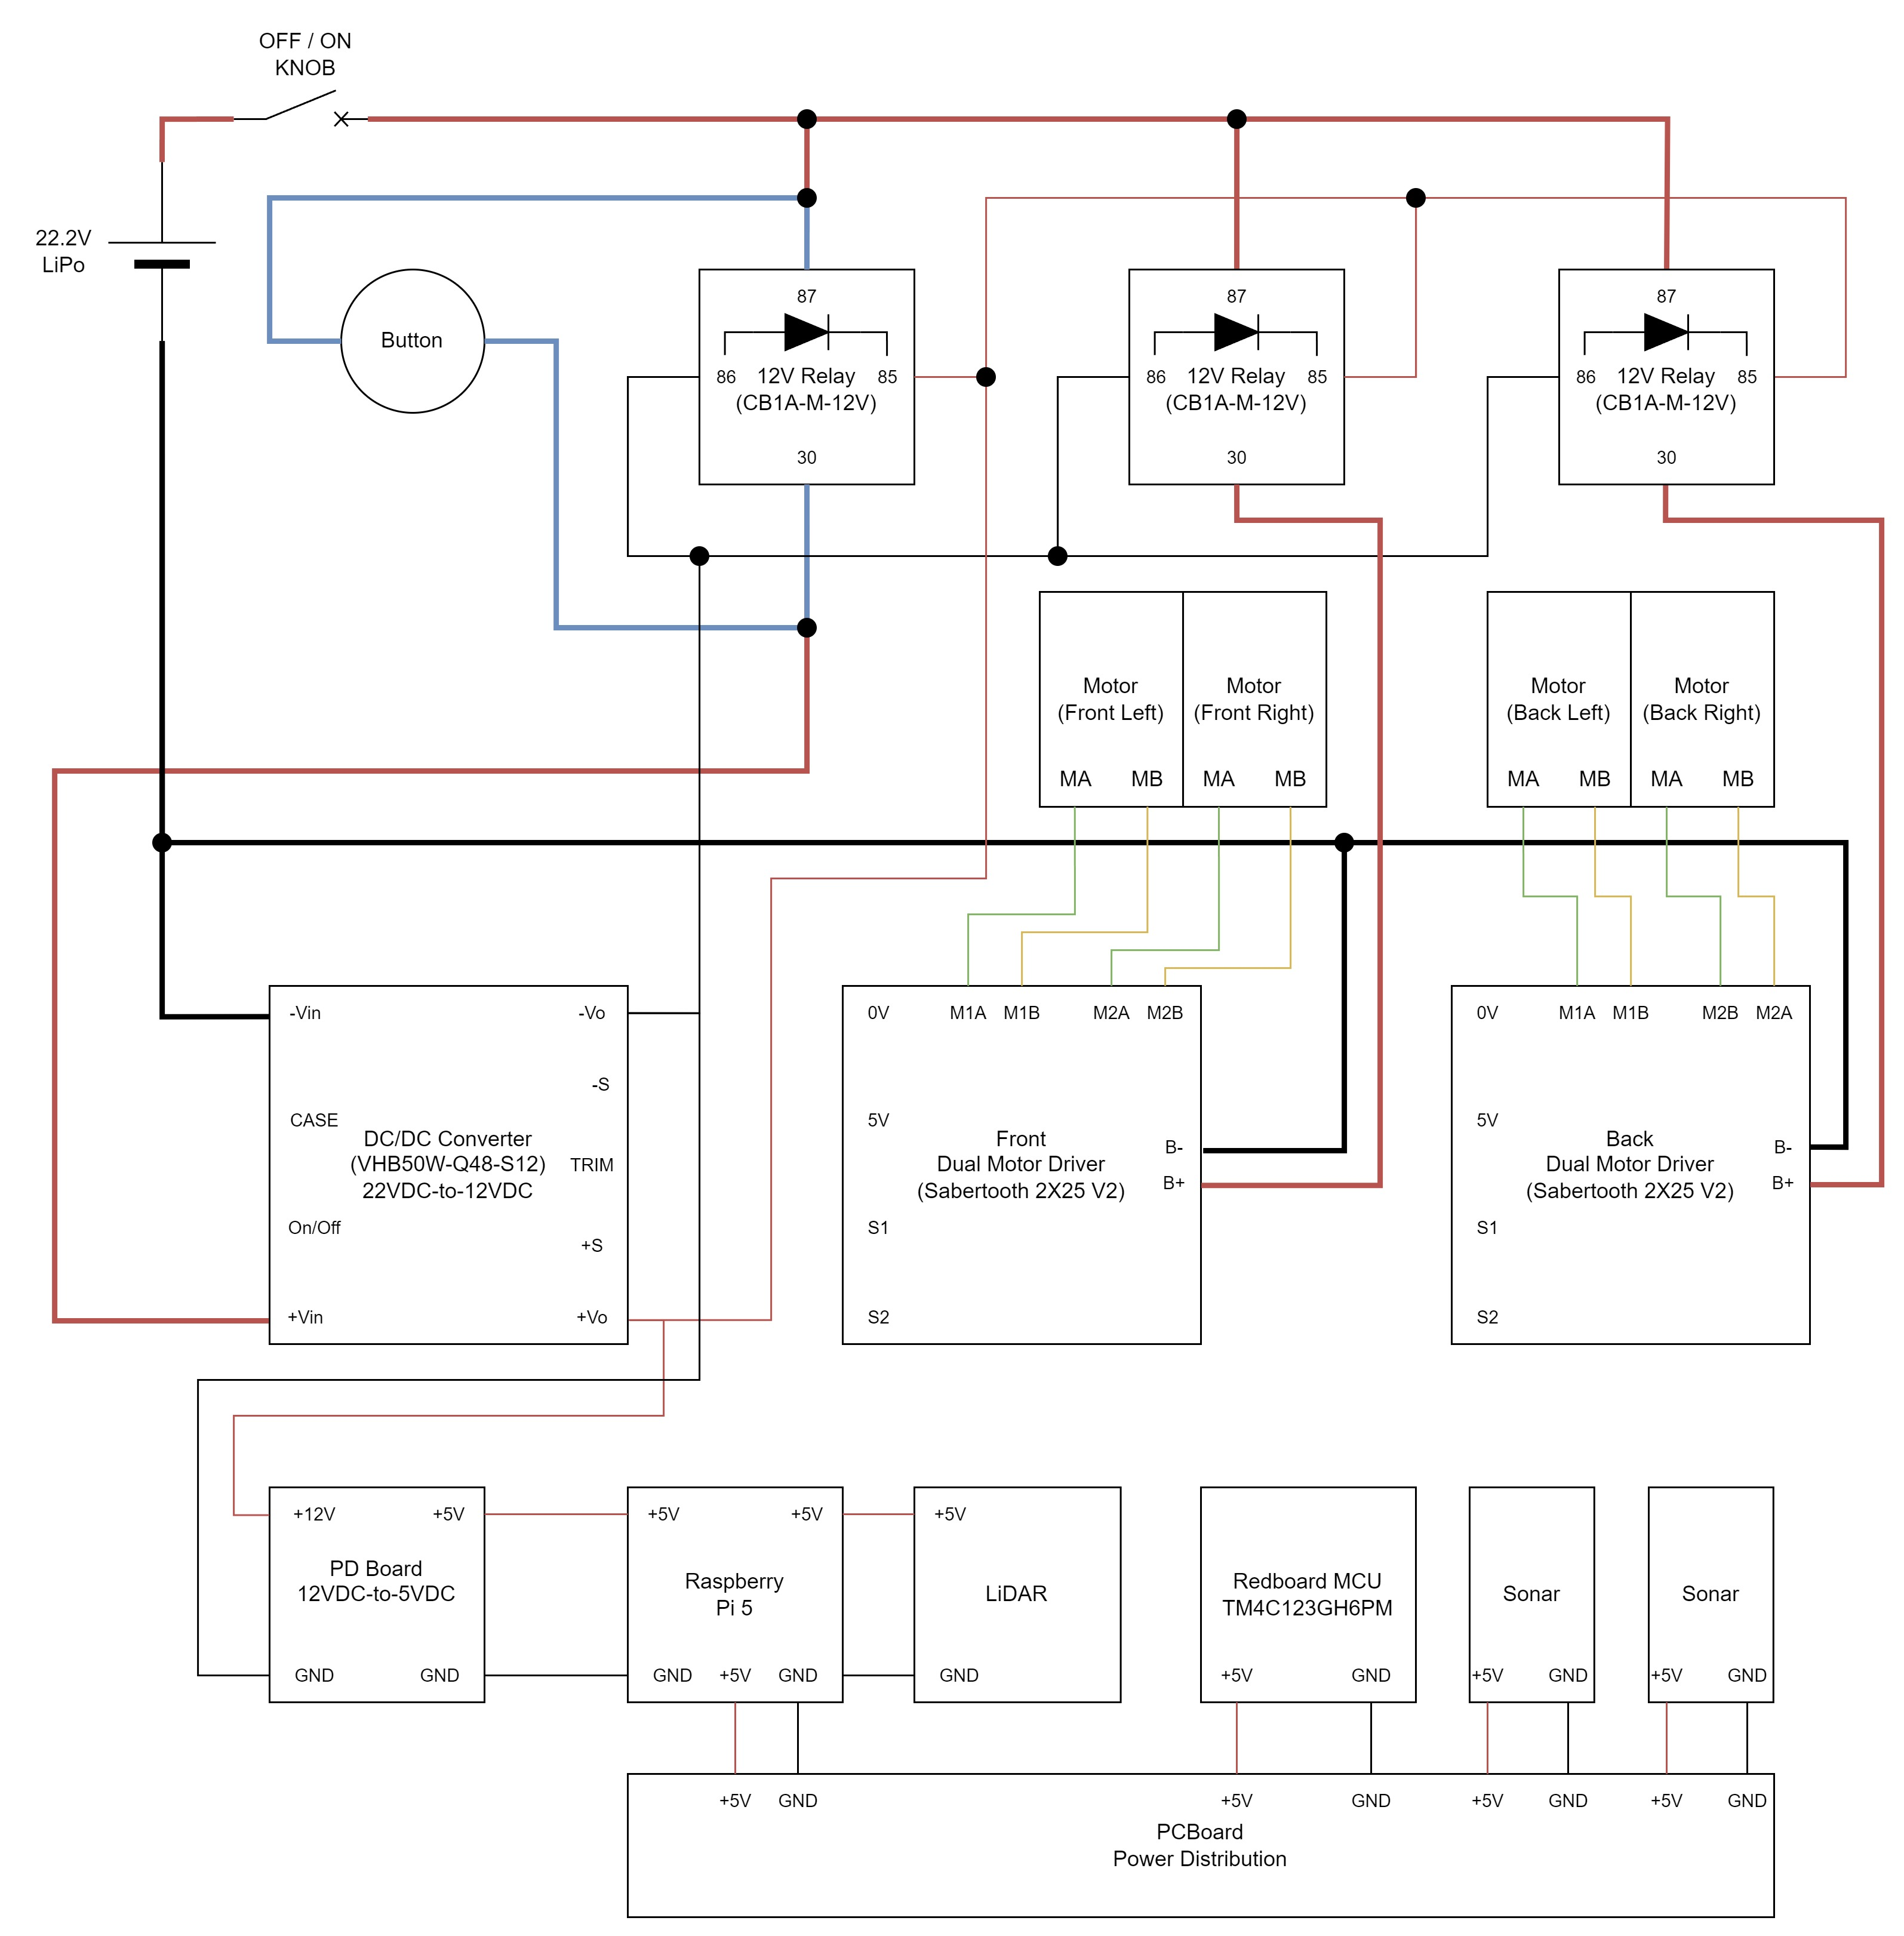
\includegraphics[width=1.00\textwidth]{images/circuits/4_power_system.jpg}
 \caption{Power System}
 \label{fig:Power System}
\end{figure}
\clearpage

%%% References
% \bibliographystyle{reference/IEEEtran_custom}
\bibliographystyle{plainurl}
\bibliography{reference/refs}{}
\end{document}